% v0.8.3 - L_k (Pointer-Chase). Content-only file; included via main.tex

\section{Target Language \texorpdfstring{$L_k$}{Lk} (Pointer-Chase)}
\label{Lk:sec:Lk}

\paragraph{Assumptions \& Regime.}
We work in the restricted regime: deterministic computation, single pass over the input, no advice, and no randomness. The $\iota$-interface is frozen by Table~\ref{tab:iota-spec} with per-step budget
\[ B(d,n) \;=\; c\,d\,\log n, \quad c\ge 1 \text{ fixed.} \]
Every computation step performs exactly one $\iota_j$ call with payload injected into the transition function that step; see Definition~\ref{def:iota-injection}. Transcript accounting follows from Lemma~\ref{lemma:budget-9-2} (Budget Lemma) and Table~\ref{tab:iota-spec}.

\paragraph{Setup and Encoding.}
Parameters: fix an integer $k\ge 2$. For a universe size $m$, the input consists of $k$ functions $T_1,\ldots,T_k : [m]\to[m]$, a tail predicate $b:[m]\to\{0,1\}$, and a designated start index $s\in[m]$ (see Remark~\ref{Lk:start-index}). The canonical bit-encoding stores each $T_j$ as an $m$-entry table with values in $[m]$ using $\lceil\log m\rceil$ bits per entry, and $b$ as $m$ bits. Thus the total input length is
\[
 n \;=\; \underbrace{k\,m\,\lceil\log m\rceil}_{\text{tables}} \; + \; \underbrace{m}_{\text{tail}} \;=\; \Theta(k\,m\log m).
\]
Equivalently, for fixed $k$, we will use $m = \Theta(n/k)$, and we keep constants explicit until the final $\Omega(\cdot)$ line.

\begin{remark}[Start index size]\label{Lk:start-index}
Including the starting index $s\in[m]$ into the input description changes the total input length by at most $O(1)$ bits and does not affect any asymptotic bounds used below.
\end{remark}

\begin{definition}[Language $L_k$]
Let $u_0 := s$ and, for $j\in\{1,\ldots,k\}$, define $u_j := T_j(u_{j-1})$. The machine accepts the input iff $b(u_k)=1$. We denote this language by $L_k$.
\end{definition}

\begin{remark}[Canonical lower-bound tools]
We refer to the following canonical tools throughout:
\begin{itemize}
  \item Lemma~\ref{lemma:budget-9-2} (Budget Lemma) and Table~\ref{tab:iota-spec}
  \item $\Psi$--Fooling Bound (Theorem~\ref{Lk:psi-fooling})
  \item $\Psi$--Fano Bound (Lemma~\ref{Lk:psi-fano})
\end{itemize}
\end{remark}


\begin{remark}[Aliases for $\Psi$--Fooling and $\Psi$--Fano]\label{Lk:aliases}
Within this section, we refer to the canonical statements in the lower-bound tools as $\Psi$--Fooling (Theorem~\ref{Lk:psi-fooling}) and $\Psi$--Fano (Lemma~\ref{Lk:psi-fano}).
\end{remark}

\begin{lemma}[Single-Pass Access for $L_k$]\label{Lk:single-pass}
In the restricted regime (deterministic, one-pass, no-advice, no-randomness) with $\iota$-interface $B(d,n)=c\cdot d\log n$, the encoding layout $T_1\parallel T_2\parallel\cdots\parallel T_k\parallel b$ admits a single-pass evaluation strategy: in phase $j$, the index $u_{j-1}$ is maintained using $O(\log m)$ workspace; exactly one $\iota_j$-call is made per step, and no random access across blocks is required.
\end{lemma}

\begin{theorem}[UB at depth $k$]\label{Lk:ub-main}
Assume the restricted regime (deterministic, single pass, no advice, no randomness) and Table~\ref{tab:iota-spec}. There exists a depth-$k$ $\Psi$-algorithm deciding $L_k$ in time $O(n)$ and workspace $O(\log m)$. The proof follows the phase-by-phase single-pass strategy of Lemma~\ref{Lk:single-pass}.
\end{theorem}

\begin{proof}
We execute a $k$-phase sequential scan of the input, conforming to the one-pass constraint. In Phase $j\in\{1,\dots,k\}$ we read the table of $T_j$ left-to-right and maintain a single index register storing $u_{j-1}\in[m]$ and its update to $u_j=T_j(u_{j-1})$. During Phase $j$, each computation step uses exactly one $\iota_j$ call per step to inject the per-step payload into $\delta$, enabling selectors-only access to any permitted local view (Table~\ref{tab:iota-spec}); in particular, this enforces the per-step information bound $B(d,n)=c\,d\,\log n$ without exceeding it. No random access is needed: we compute $u_j$ by a single pass over the $T_j$ table, updating the index when the row for $u_{j-1}$ is encountered.

After completing Phase $k$, we scan the $b$ array once and read $b(u_k)$ at the designated position. Accounting: each phase scans a disjoint $\Theta(m\log m)$-bit block once, so total I/O is $O(n)$. The workspace keeps only the current phase counter, the index $u_j$ and constant-many loop variables, which is $O(\log m)$ bits. Preconditions are satisfied and the per-step $\iota$ usage complies with Table~\ref{tab:iota-spec}.
\end{proof}

\begin{lemma}[Fooling family for $L_k$]
\label{Lk:lem:fooling-Lk}
There exists a family $\{\mathcal{F}_n\}_n$ with $\lvert\mathcal{F}_n\rvert = 2^{\alpha m}$ for a constant $\alpha>0$, such that any depth-$(k{-}1)$ $\Psi$-algorithm in the restricted regime produces identical transcripts on distinct $x,x'\in\mathcal{F}_n$ while the answers differ via $b(u_k)$.
\end{lemma}

\begin{proof}
Fix $T_1,\ldots,T_{k-1}$ and fix any subset $S\subseteq[m]$ of size $\lvert S\rvert \ge 0.9\,m$. Consider instances that agree on all components except on $(T_k\upharpoonright S,\, b\upharpoonright S)$; within $S$, vary $T_k$ and $b$ arbitrarily. Under the restricted regime and budget $B(k{-}1,n)=c\,(k{-}1)\,\log n$ (Table~\ref{tab:iota-spec}), any depth-$(k{-}1)$ machine that runs for fewer than $T$ steps can see at most $T\cdot B(k{-}1,n)$ bits across the entire computation by Lemma~\ref{lemma:budget-9-2} (Budget Lemma). For appropriate $T=o(m)$, the final-layer degrees of freedom on $S$ dominate, so there exist distinct $(T_k,b)$ and $(T_k',b')$ in this family that induce identical transcripts yet route $u_k$ into positions with different $b$-labels. Hence $\lvert\mathcal{F}_n\rvert \ge 2^{\alpha m}$ for some constant $\alpha\in(0,1)$; in particular we can take $\alpha\approx 0.9$ by construction. This is the standard last-layer entropy argument adapted to the $\Psi$-budgeted setting.
\end{proof}

\begin{theorem}[LB at depth $k{-}1$]\label{Lk:lb-main}
Assume the restricted regime and Table~\ref{tab:iota-spec}. Any depth-$(k{-}1)$ $\Psi$-algorithm deciding $L_k$ requires
\[
 T(n) \;=\; \Omega\!\left(\frac{n}{k\,(k{-}1)\,\log n}\right).
\]
\end{theorem}

\begin{proof}
By Lemma~\ref{Lk:lem:fooling-Lk}, there is a fooling family of size $|\mathcal{F}_n| = 2^{\alpha m}$ with $\alpha>0$ and $m=\Theta(n/k)$. Applying the $\Psi$--Fooling Bound (Theorem~\ref{thm:psi-fooling}) at depth $(k-1)$ and using Lemma~\ref{lemma:budget-9-2} (Budget Lemma) and Table~\ref{tab:iota-spec} yields
\[
 T \;\ge\; \frac{\log|\mathcal{F}_n|}{B(k-1,n)} \;=\; \frac{\alpha\,m}{c\,(k-1)\,\log n} \;=\; \Omega\!\left(\frac{n}{k\,(k-1)\,\log n}\right),
\]
keeping $c$ and $\alpha$ explicit until the asymptotic form. In particular, $T \ge \alpha m / ( c (k-1) \log n )$. Here constants $\alpha,c>0$ are absorbed into the $\Omega(\cdot)$ notation.
\end{proof}

\IfFileExists{paper/fig/lk_logM.png}{%
\begin{figure}[t]
  \centering
  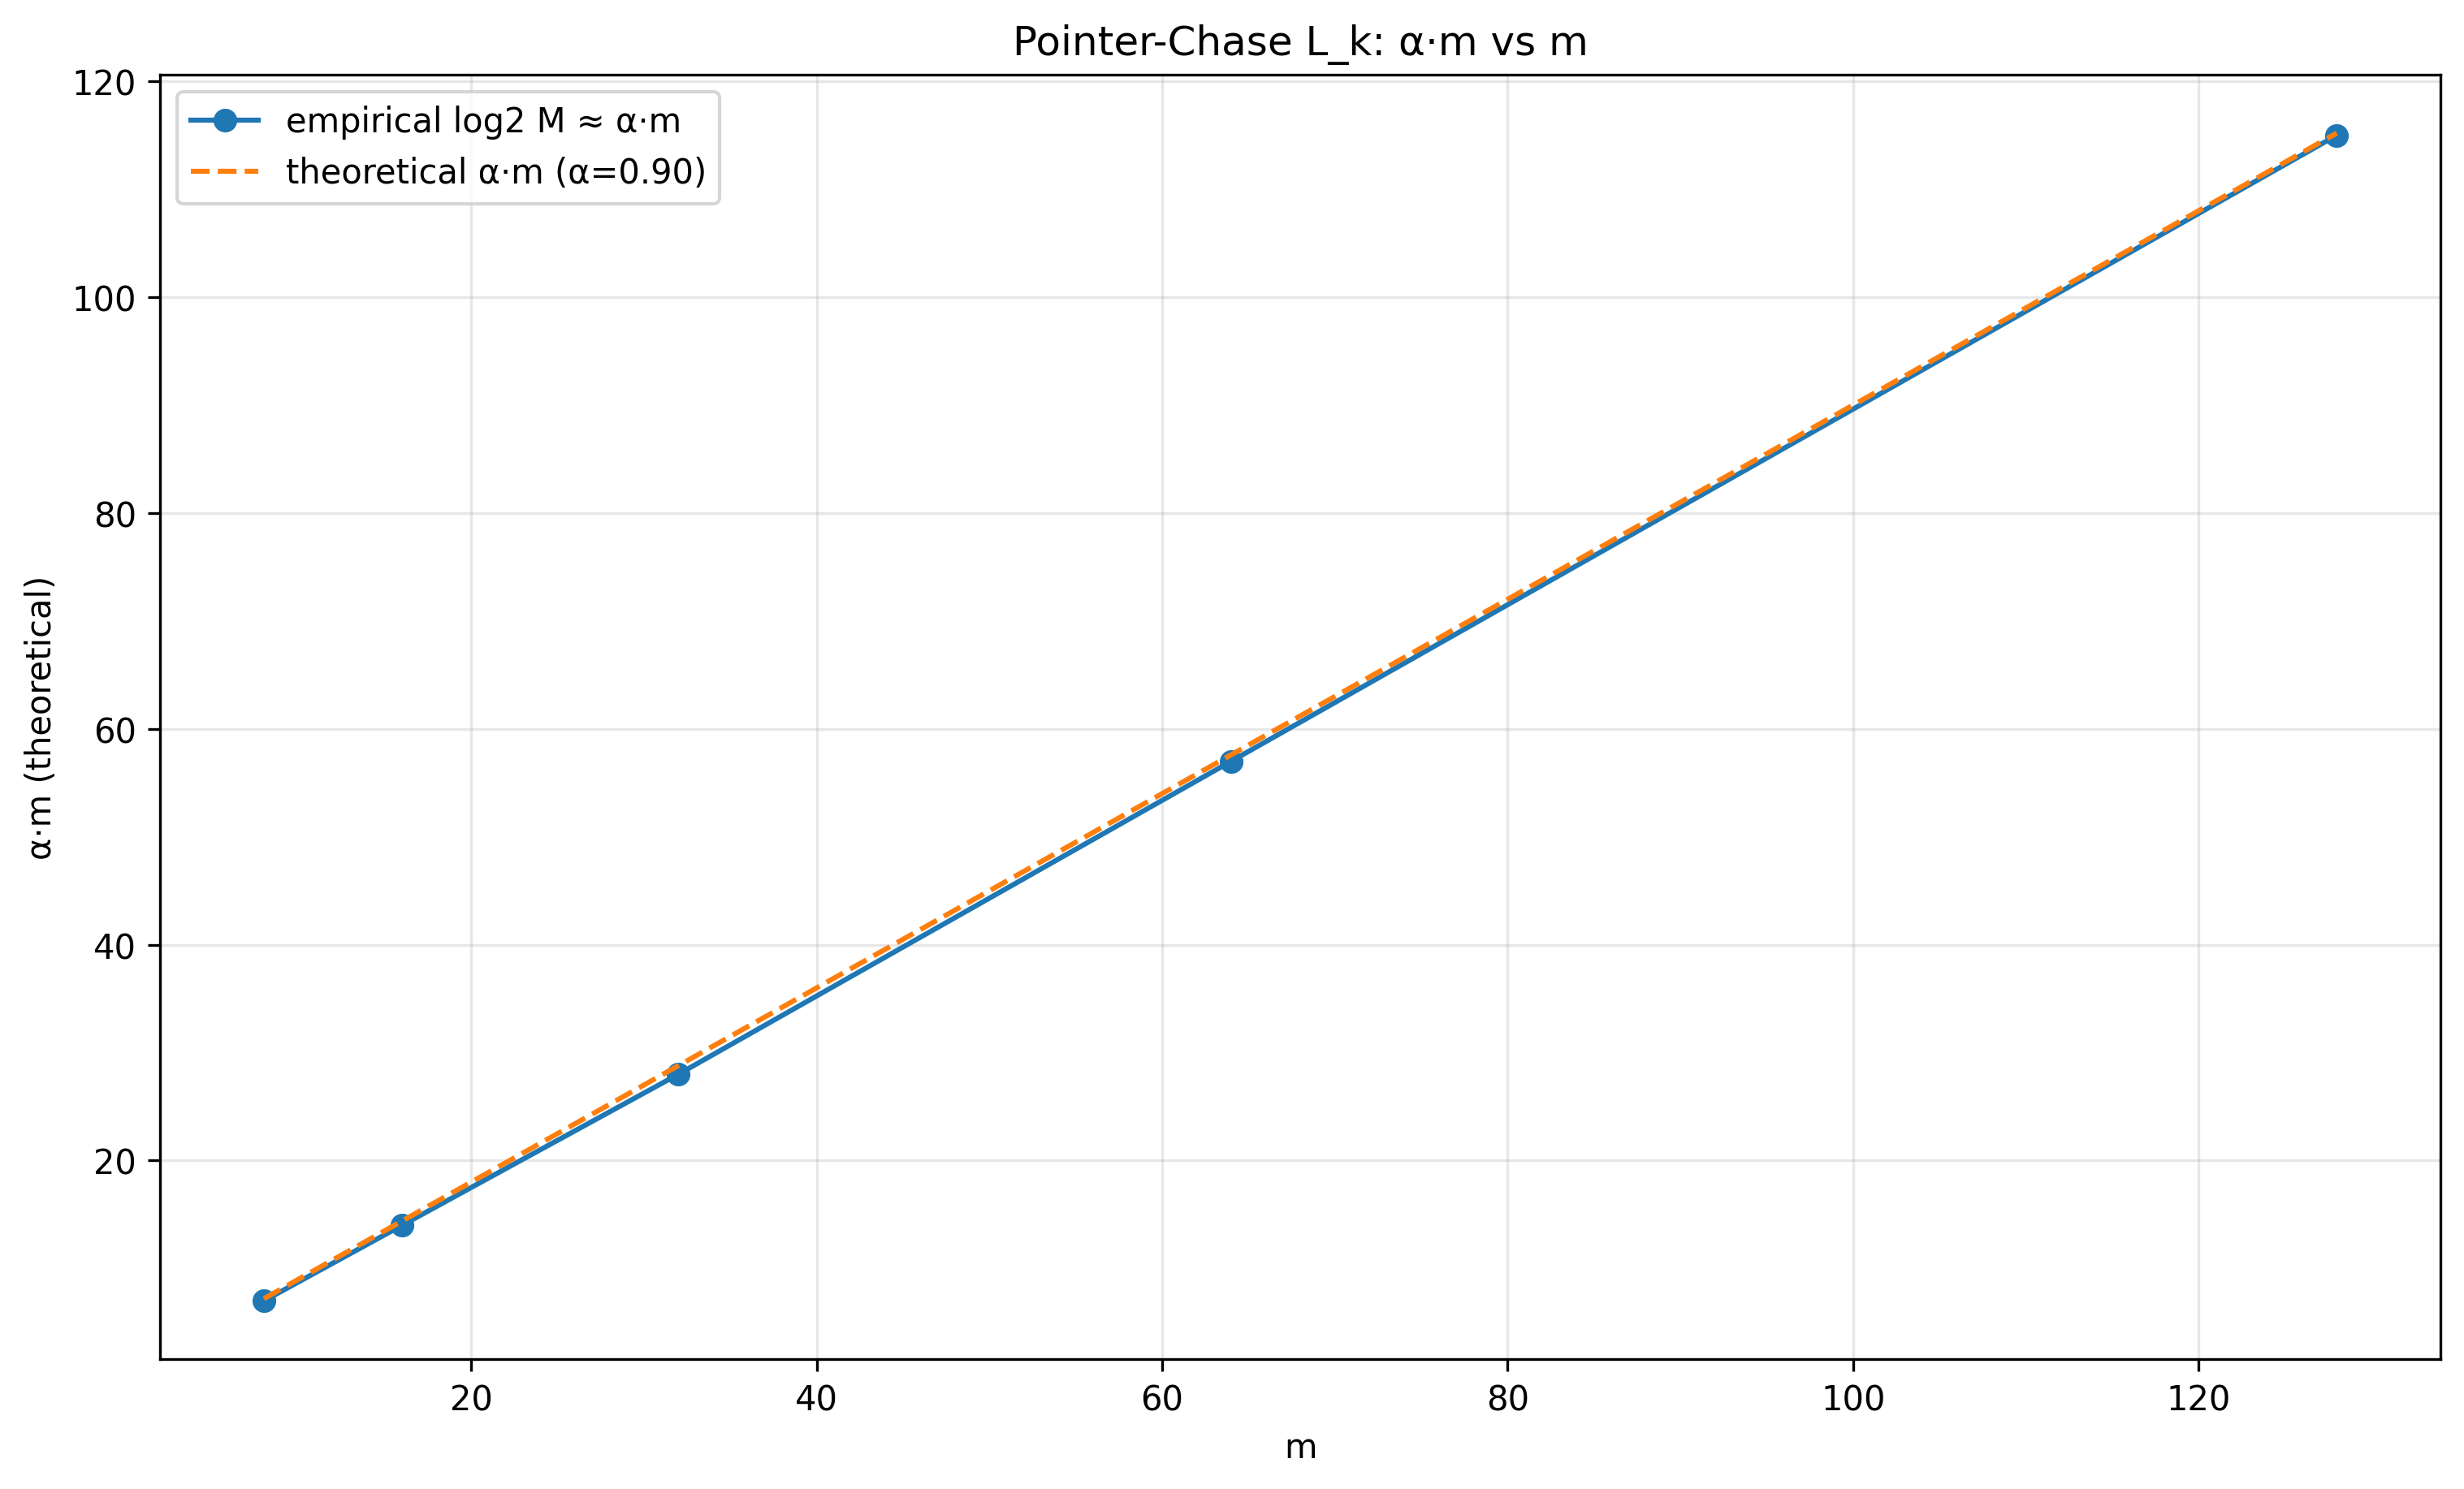
\includegraphics[width=\linewidth]{paper/fig/lk_logM.png}
  \caption{Trendline for $\alpha\cdot m$ vs.\ $m$ (Pointer-Chase).}
  \label{Lk:fig-lk-logM}
\end{figure}
}{%
\noindent The expected trend is linear in $m$, i.e., $y=\alpha\cdot m$ (log-scale visualization omitted in this version).%
}

\paragraph{Anti-Simulation Preview.}
\begin{remark}[Average-case via $\Psi$--Fano]\label{Lk:avg-fano}
For average-case instances of $L_k$, combining the same budget accounting with $\Psi$--Fano (Lemma~\ref{Lk:psi-fano}) yields the standard mutual-information bound; we do not pursue the optimization here, as our focus is the worst-case separation.
\end{remark}
In version 0.8.5 (planned), we intend to formalize the following: depth $(k{-}1)$ cannot polynomially simulate depth $k$ even with transcript access bounded by $B(d,n)$, since the final-layer entropy revealed only at depth $k$ cannot be recovered within the $(k{-}1)$ budget. This will be stated as an anti-simulation lemma: any attempt to inline the last layer either forces superlinear I/O or violates the per-step $\iota$ policy. For the full statement and proof strategy, please refer to version 0.8.5 when it becomes available.

